\documentclass{beamer}
\usepackage[utf8]{inputenc}
\usepackage[T1]{fontenc}
\usepackage{lmodern}
\usepackage{tikz}
\usetikzlibrary{math}
\usetikzlibrary{snakes}
\usetikzlibrary{decorations.pathreplacing}
\usepackage[absolute,overlay]{textpos}
\usepackage{booktabs}
\usepackage{ulem}
\usepackage{array}

\title{Abschlusspräsentation}
\author{Projektgruppe FastSense}
\date{11. März 2021}

\usecolortheme{seahorse}
\definecolor{dark}{rgb}{0, 0.1, 0.3}
\definecolor{light}{rgb}{0.9, 0.933, 1}
\definecolor{hw}{rgb}{0.8, 1, 0.9}
\definecolor{red}{rgb}{1, 0, 0}
\definecolor{yellow}{rgb}{1, 1, 0}
\definecolor{green}{rgb}{0, 1, 0}
\definecolor{cyan}{rgb}{0, 1, 1}
\definecolor{blue}{rgb}{0, 0, 1}
\definecolor{magenta}{rgb}{1, 0, 1}
\definecolor{grey}{rgb}{0.8, 0.8, 0.8}
\setbeamercolor{normal text}{fg=black}
\setbeamercolor{structure}{fg=dark}
\setbeamercolor{footline}{fg=black}
\setbeamercolor{frametitle}{fg=light,bg=dark}
\setbeamertemplate{itemize items}[circle]
\beamertemplatenavigationsymbolsempty
\addtobeamertemplate{navigation symbols}{}{
    \usebeamerfont{footline}
    \usebeamercolor[fg]{footline}
    {\footnotesize \insertframenumber\\\vspace{0.15cm}}
}
\setbeamertemplate{title page}{
\insertauthor\\
\vspace{0.5cm}
\begin{LARGE}\textbf{\inserttitle}\end{LARGE}\\
\vspace{0.5cm}
\insertdate
}

\begin{document}

{\setbeamertemplate{navigation symbols}{}
\begin{frame}
\titlepage
\end{frame}}

\section{Zielsetzung}
\begin{frame}{\secname}
\begin{itemize}
\item Autonome echtzeitfähige Kartierung
\item FPGA-basierte Hardwarebeschleunigung
\item Einfaches, handliches System
\item Anbindung an bestehende Systeme (LVR2)
\end{itemize}
\end{frame}

\section{MS1: Trail Detection}
\begin{frame}{\secname}
TODO    
\end{frame}

\section{SLAM-Box}
\begin{frame}{\secname}
TODO
\end{frame}

\section{Vorgehen}
\begin{frame}{\secname}
TODO    
\end{frame}

\section{TSDF}
\begin{frame}{\secname}
\begin{center}
\includegraphics[width=5cm]{images/TSDF_Gen_new.png}
\includegraphics[width=5cm]{images/TSDF_3D.png}
\end{center}
\end{frame}

\section{Point-to-TSDF Registrierung}
\begin{frame}{\secname}
\begin{center}
\includegraphics[width=7cm]{images/Reg_Gradient.png}
\includegraphics[width=7cm]{images/Pose_Graph.png}
\end{center}
\end{frame}

\section{Hardware Architektur}
\begin{frame}{\secname}
\begin{center}
\includegraphics[width=10cm]{images/Blockdiagram.pdf}
\end{center}
\end{frame}

\section{Aufbau}
\begin{frame}{\secname}
\begin{textblock*}{5.8cm}(1cm,1.1cm)
\centering
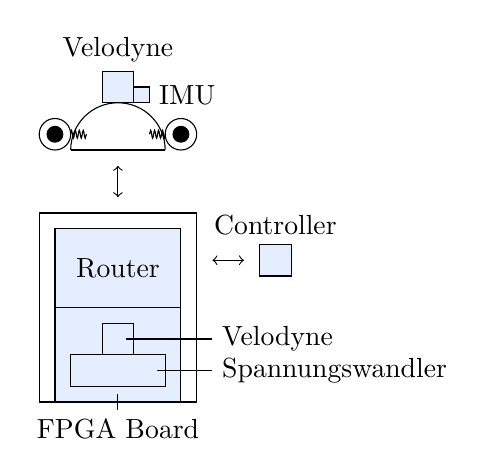
\begin{tikzpicture}[scale=0.4]
\draw (3, 10) arc (0:180:1.5);
\draw (0, 10) -- (3, 10);
\draw[fill=light] (1, 11.5) rectangle +(1, 1);
\node[above] at (1.5, 12.5) {Velodyne};
\draw[fill=light] (2, 11.5) rectangle +(0.5, 0.5);
\node[right] at (2.5, 11.75) {IMU};
\draw [decorate, decoration={snake, segment length=0.5mm, amplitude=0.5mm}]
(0.5, 10.5) -- (-0.5, 10.5);
\draw [fill=white] (-0.5, 10.5) circle (0.5);
\draw [fill=black] (-0.5, 10.5) circle (0.25);
\draw [decorate, decoration={snake, segment length=0.5mm, amplitude=0.5mm}]
(2.5, 10.5) -- (3.5, 10.5);
\draw [fill=white] (3.5, 10.5) circle (0.5);
\draw [fill=black] (3.5, 10.5) circle (0.25);
\draw (-1, 2) rectangle +(5, 6);
\draw[fill=light] (-0.5, 2) rectangle +(4, 3);
\draw (1.5, 2.25) -- (1.5, 1.75) node[below] {FPGA Board};
\draw[fill=light] (1, 3.5) rectangle +(1, 1);
\draw (1.75, 4) -- (4.5, 4) node[right] {Velodyne};
\draw[fill=light] (0, 2.5) rectangle +(3, 1);
\draw (2.75, 3) -- (4.5, 3) node[right] {Spannungswandler};
\draw[fill=light] (-0.5, 5) rectangle +(4, 2.5)
node[pos=0.5] {Router};
\draw[fill=light] (6, 6) rectangle +(1, 1);
\node[above] at (6.5, 7) {Controller};
\draw[<->] (1.5, 8.5) -- (1.5, 9.5);
\draw[<->] (4.5, 6.5) -- (5.5, 6.5);
\end{tikzpicture}
\end{textblock*}
\begin{textblock*}{5.8cm}(1cm,6.7cm)
\centering
\includegraphics[width=3.5cm]{images/Box.jpg}
\end{textblock*}
\begin{textblock*}{5cm}(6.8cm,1.1cm)
\includegraphics[width=5cm]{images/Rucksack02.jpg}
\includegraphics[width=5cm]{images/Rucksack01.jpg}
\end{textblock*}
\end{frame}

\section{Evaluation}
\subsection{Zeit}
\begin{frame}{\secname: \subsecname}
\begin{textblock*}{12.8cm}(0cm, 1.1cm)
\centering
\definecolor{bad}{rgb}{1, 0.5, 0.4}
\begin{tikzpicture}[scale=0.85]
\draw[->] (0, 0) -- (10.5, 0) node[right] {Zeit [ms]};
\draw[->] (0, 0) -- (0, 8) node[above] {Anzahl Scans};
\foreach \i\y in {0/3,1/11,2/15,3/10,4/7,5/3,6/2,7/1,8/1,9/1} {
    \pgfmathsetmacro\x{int(\i * 10)}
    \draw (\i, -0.1) node[below]{\x} -- (\i, 0.1);
    \tikzmath {
        if {\i < 5} then {
            let \c = light;
        } else {
            let \c = bad;
        };
        { \draw[fill=\c] (\i, 0) rectangle (\i+1, \y/2); };
    }
}
\draw (9.5, 0.25) -- (9.5, -0.5) node[below] {$>90$};
\node[below right] at (6, 8) {\begin{minipage}{6cm}
\begin{itemize}
\item{6. Stock WB; 8000 Scans; \\
$\varepsilon$ = 0,04}
\item{Avg: 30\,ms}
\item[\color{bad}$\bullet$]{11\% aller Scans über 50\,ms}
\item[\color{red}$\bullet$]{2\% gedroppt $\Rightarrow$ 19,6\,fps}
\end{itemize}
\end{minipage}};
\end{tikzpicture}
\end{textblock*}
\end{frame}

\begin{frame}{\secname: \subsecname}
\begin{textblock*}{12.8cm}(0cm, 1.1cm)
\centering
\definecolor{bad}{rgb}{1, 0.5, 0.4}
\begin{tikzpicture}[scale=0.85]
\draw[->] (0, 0) -- (10.5, 0) node[right] {Zeit [ms]};
\draw[->] (0, 0) -- (0, 8) node[above] {Anzahl Scans};
\foreach \i\y in {0/1,1/5,2/7,3/8,4/8,5/14,6/7,7/3,8/1,9/2} {
    \pgfmathsetmacro\x{int(\i * 10)}
    \draw (\i, -0.1) node[below]{\x} -- (\i, 0.1);
    \tikzmath {
        if {\i < 5} then {
            let \c = light;
        } else {
            let \c = bad;
        };
        { \draw[fill=\c] (\i, 0) rectangle (\i+1, \y/2); };
    }
}
\draw (9.5, 0.25) -- (9.5, -0.5) node[below] {$>90$};
\node[below right] at (6, 8) {\begin{minipage}{6cm}
\begin{itemize}
\item{6. Stock WB; 6000 Scans; \\
$\varepsilon$ = 0,01}
\item{Avg: 47\,ms}
\item[\color{bad}$\bullet$]{48\% aller Scans über 50\,ms}
\item[\color{red}$\bullet$]{10\% gedroppt $\Rightarrow$ 18\,fps}
\end{itemize}
\end{minipage}};
\end{tikzpicture}
\end{textblock*}
\end{frame}    

\subsection{Power Consumption}
\begin{frame}{\secname: \subsecname}
\centering
\includegraphics[width=8cm]{images/power_consumption.jpg}\\\vspace{0.5cm}
\begin{tabular}{lllllll}
\toprule
& \multicolumn{3}{c}{Idle} & \multicolumn{3}{c}{Running} \\
& Mean & Min & Max & Mean & Min & Max \\
\midrule
U [mV] & 78,7 & 76 & 88 & 89,8 & 85,7 & 105,5 \\
I [A] & 1,124 & 1,086 & 1,257 & 1,283 & 1,224 & 1,507 \\
P [W] & 13,488 & 13,032 & 15,084 & \textbf{15,396} & 14,688 & 18,084 \\
\bottomrule
\end{tabular}
\end{frame}

\subsection{Genauigkeit}
\begin{frame}{\secname: \subsecname}
\begin{itemize}
\item{6. Stockwerk (Distanzabweichung in Meter)}
\begin{center}
\begin{tabular}{ccc}
\toprule
$\varepsilon$ & 0,01 & 0,04 \\ 
\midrule
& 0,0615 & 0,0505 \\  
\bottomrule
\end{tabular}
\end{center}
\begin{center}
\begin{tabular}{ccc}
\toprule
Geschw. & langsam & schnell \\ 
\midrule
& 0,0505 & 0,0437 \\  
\bottomrule
\end{tabular}
\end{center}
\begin{itemize}
\item{gesamt (langsam, $\varepsilon$ = 0,04): 0,075349}
\end{itemize}
\item{8 Meter Labortest (Distanzabweichung in Meter)}
\begin{center}
\begin{tabular}{cccc}
\toprule
& hin & zurück & gesamt \\ 
\midrule
langsam & 0,0548 & 0,0650 & 0,0861 \\  
schnell & 0,1676 & 0,0459 & 0,1320 \\
\bottomrule
\end{tabular}
\end{center}
\end{itemize}
\end{frame}

\section{Fazit}
\begin{frame}{\secname}
\begin{itemize}
\item{Portables System}
\item{Weiche Echtzeitfähigkeit}
\item{Geringer Stromverbrauch}
\item{Einfache Handhabung}
\item{Einfache Analyse}
\end{itemize}   
\end{frame}

\section{Ausblick}
\begin{frame}{\secname}
\begin{itemize}
\item Evaluierung mit anderer Sensorik
\item Portierung auf Drohne
\item Optimierung des Posegraphen (Loop Closing)
\item Paper
\end{itemize}
\end{frame}

\end{document}
